\documentclass{article}
\usepackage[utf8]{inputenc}
\usepackage{amsmath}
\usepackage{amsfonts}
\usepackage{amssymb}
\usepackage{graphicx}
\usepackage{tabularx}
\usepackage{caption}
\usepackage{subcaption}
\title{\Huge {\textbf{\textit{\emph{Transportation Congestion}}}}}
\date{}
\author{\huge{Team FCI }\\\\\\  \huge{faculty of Computer \& Information} \\\\\\  \huge{Level 2}}
\begin{document}
\maketitle
\newpage
\section{Problem:} 
 The means of transportation nowadays are a great blessing that Allah has bestowed on man. These methods help to approximate distances, reduce waste time on road between starting points for trips and destination. But there are many negative phenomena and problems related to transportation, especially land transport, and perhaps the most prominent of these phenomena is the traffic congestion, which makes some streets seem to be large places for car parking. In addition to the fact that congestion has very negative effects on the human psyche, hence the government solution to the
problem of traffic jams is a top priority. perhaps the most important effects of this negative phenomenon:
\subsection{Effects}
 
\begin{itemize}
  \item Infection with infectious diseases, especially when we are in the days of 
Corona The number was either in car parks or trains, etc...
  \item Steam trains and some other types of road transport expose theatmosphere 
to the risk of pollution due to the smoke rising from them.
  \item This phenomenon caused an increase in pollution rates due to the spread of 
diseases
  \item High rates of infection with some diseases resulting from lack of 
movement,due to the great dependence of people on means of transportation 
to move from one place to another, even if the distance is very short, and the 
person does not need to use his own vehicle. 
  \item Traffic congestion is increasing in the streets, which hinders people 
fromreaching their destinations at the required and specified times.
  \item It also caused a lot of noise in the cities, which led to the 
population’sannoyance.
\end{itemize}
\begin{figure}[!h]
  
    \begin{subfigure}[!h]{0.40\columnwidth}
      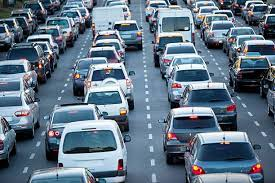
\includegraphics{traffic.jpg}
       \caption{this 1 subfigure}
        \label{sfig 1}
     \end{subfigure}
~
     \begin{subfigure}[!h]{0.40\columnwidth}
      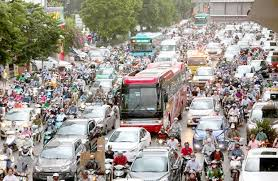
\includegraphics{traffic 2.jpg}
       \caption{this 2 subfigure}
        \label{sfig 2}
      \end{subfigure}
\caption{traffic jam}
\end{figure}


\newpage

\section{Solution:}
\begin{enumerate}
  \item  Build an application to solve the problem of traffic congestion. 
  \item There are laws regulating the movement of cars. 
  \item Establish strict controls for workers to leave their establishments during 
official working hours. 
  \item Increasing 
the number of internal means to reduce this severe overcrowding.
  \item Using individual transportation more than mass transit. 
\end{enumerate}
\section{APP Features:}
\begin{itemize}
  \item Make an application to request a private car or reserve places in the cars 
responsible for moving between cities and universities for students (this is the 
idea of our project). 
\end{itemize}

\begin{figure}[!h]
   \centering
   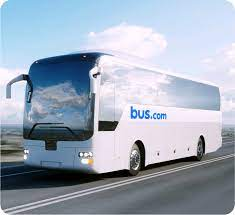
\includegraphics{bus.jpg}
   \caption{app}
   \label{fig : app features}
\end{figure}

\begin{itemize}
\item In our app we collect information about the most crowded cities in the 
stateand regulate the movement of cars . 
\item  We will also add some regulations for workers to leave 
theirestablishments. This is by making people aware of the regularity at 
work and respecting the times of leaving their organizations it will also be 
attached by some videos.
\item we will also make use of google maps to help us to find people in same area 
\item The app also asks you which place in the car you want to reserve and if you 
are patient or disapled you can reserve a private car . 
\item Make it easy to open and download our app .
\item App also includes options for rating the service and the drivers. 
\item App will save time by choosing quickest route and provide service 24 hours a 
day.
\end{itemize}

\begin{table}
\centering
\begin{tabular}{|c|c|c|}
\hline 
\multicolumn{3}{|c|}{Work Time}\\
\hline
Day & From & To \\ 

\hline 
Sunday &8:00 am  & 5:00 pm \\ 
\hline 
Monday & 8:00 am & 5:00 pm  \\ 
\hline 
Tushday & 8:00 am &5:00 pm  \\ 
\hline 
Wednesday& 8:00 am &5:00 pm  \\ 
\hline 
Thursday & 8:00 am &5:00 pm  \\ 
\hline 
Friday&\multicolumn{2}{|c|}{Week End}\\
\hline 
Saturday & 8:00 am & 2:00 pm \\
\hline
\end{tabular} 
\caption{work time}\label{t1}
\end{table}
\newpage


\begin{table}
\centering
\begin{tabular}{|c|c|c|}
\hline 
\multicolumn{3}{|c|}{Team Members}\\
\hline
First Name & Second Name & Seaction Number \\ 
\hline 
Nahla &Mohamed Saeed & Sec 10 \\ 
\hline 
Hessain & EL-Sid & Sec 3  \\ 
\hline 
Ramadan & Adham Ali &Sec 11\\ 
\hline 
Mohamed& Hamdey &Sec 11  \\ 
\hline 
Ahmad& AL-Shahawy &Sec 11 \\ 
\hline 
NorEL-Deen&kamel&Sec \\
\hline
\end{tabular} 
\caption{Information about team members}\label{t2}
\end{table}
\newpage
\begin{center}
\Huge {\textbf{\textit{\emph{Thanks}}}}
\end{center}
\end{document}